\section{目的}
依據 \textit{AIC Lab.pdf} PDF 22--30 頁，完成分壓型、threshold self-bias 與含啟動電路的電壓參考，觀察供應電壓及溫度敏感度。使用由使用者另行提供的模型庫，供應電壓為 1.0 V。這是本次教學適配條件，並非模型額定電壓的認證；講義原製程的 3.3 V 圖表與數字不直接當作通過門檻。程式依講義拓樸重寫，原始程式僅作尺寸與缺漏的參考。

\section{Spec 對照}
S 表示在明列適配條件下已實際模擬；D 表示已回答推導或討論；L 表示原數值或完整驗證仍有限制。D01 等為檔名的數字前綴。
\small\begin{longtable}{p{.46\linewidth}p{.30\linewidth}p{.15\linewidth}}\toprule
要求與 PDF 頁碼 & 對應 deck／檢查 & 狀態 \\ \midrule\endhead
二 MOS 分壓與手算比較（22--23） & D01; DC, line AC & S+D \\
三 MOS 雙電壓、改尺寸、獨立 well（24） & D02; three sizes & S+D \\
Threshold self-bias、兩支路條件、零電流解（25） & D03; two R values & S+D \\
Startup 功能與啟動注入（26--27） & D04; ramp and disconnect & S+D \\
電流設定、自偏壓、完整 Vbias（27--29） & D05--06; DC/AC/transient & S+D \\
製程補償與溫度設計（30） & D05--06; -20/27/85 C & S+D/L \\
舊 0.8/2.1 V 與約 1.62 V 範例（24,29） & 1 V adaptation & L \\
\bottomrule\end{longtable}\normalsize


\section{電路與設計推導}
\[
\beta_n(V_{ref}-V_{Tn})^2=\beta_p(V_{DD}-V_{ref}-|V_{Tp}|)^2,
\quad
V_{ref}\simeq\frac{V_{DD}-|V_{Tp}|+\sqrt{\beta_n/\beta_p}V_{Tn}}{1+\sqrt{\beta_n/\beta_p}}.
\]
\[
I_{threshold}=\frac{V_{GS1}}{R},\qquad
I_{bias}\simeq\frac{2}{\beta R_b^2}\left(1-\frac{1}{\sqrt K}\right)^2,
\qquad V_{bias}=\left(1+\frac{R_3}{R_4}\right)V_{GSn}-|V_{SGp}|.
\]上式是強反轉、長通道及匹配支路的近似；$\beta$ 應屬於實際電阻退化支路中的元件極性。PDF 27 的 $\mu_n$ 不能直接套到 PDF 28 的 PMOS 電阻支路；此處 $K$ 為對應 PMOS 的尺寸比。模型含 body effect、有限輸出導納與漏電，沒有將舊製程的常數搬入本次數值計算。

D01 保留 $W_n/W_p/L=21/10/0.3\,\mu$m，修正 PMOS bulk 接地；另測 $W_p=20\,\mu$m 或 $W_n=42\,\mu$m。D02 保留兩顆 PMOS 各 $20/0.3\,\mu$m 與 NMOS $17.5/0.3\,\mu$m，另將 PMOS 或 NMOS 寬度加倍。中間 PMOS 的 body 與 source 同接，可在獨立 N-well 實現；需承擔 well 面積及隔離規則。

D03 回復原碼缺少的 M5 複製支路，$R=5/10$ k$\Omega$，輸出固定 0.5 V。M2 的 NMOS bulk 採接地，保留 body effect；若要 body-source 相接，需要另行確認隔離 well 製程。\texttt{.nodeset} 僅選擇求解起點，不是硬體啟動。

D04--06 使用講義 MS1--MS3 啟動支路與四 MOS 核心，並把原來從 1 V 開始的正弦供應改為從零上升的 PWL。完整電路 $R_b=1$ k$\Omega$、$R_3/R_4=5/1$ k$\Omega$；D05 另測 $R_3=3$ k$\Omega$ 及 $R_b=2$ k$\Omega$。

\section{模擬設定}
使用 PrimeSim HSPICE S-2021.09 win64，基本溫度 27 $^\circ$C，\texttt{runlvl=5}、\texttt{accurate}，輸出 \texttt{.op/.print/.measure}。每個 \texttt{.alter} 先重設完整基準參數與溫度，防止前一案例殘留。實際工作已完成，未出現 error 或 failed 量測；模型仍有被抑制的警告訊息，因此不宣稱完全沒有 warning。公開 netlist 不含模型路徑，以下註解標示本機執行前必須設定的模型入口；模型檔與設定只保留本機：
\begin{verbatim}
* MODEL_SETUP_REQUIRED
\end{verbatim}
CSV 與數值摘要位於該 lab 的 \texttt{results/}；所有圖均由真實列印數據重繪，不是波形軟體畫面截圖。\texttt{manifest.json} 提供 spec 對照與案例定義。本 lab 為六份 deck、22 個案例。D01--03 掃供應電壓並量測 1 Hz 的供應至輸出增益；D04 使用 1/30 $\mu$s ramp、50 $\mu$s 觀察窗；D06 觀察 100 $\mu$s，最大步距 20 ns 並用 UIC 由零電荷開始。$t_{1\%}$ 從供應開始上升計算，要求後續所有樣點保持在最終值的 1\% 內；此為本報告定義，並非講義保證。

\section{結果與規格檢查}
\begin{center}\small\begin{tabular}{lrrrr}\toprule
Case & $V_{ref1}$ (V) & $V_{ref2}$ (V) & $dV_o/dV_{DD}$ & $P_b$ ($\mu$W) \\ \midrule
D01/C0 & 0.403 & -- & 0.273 & 99.87 \\
D01/C1 & 0.432 & -- & 0.316 & 163.03 \\
D01/C2 & 0.375 & -- & 0.239 & 119.20 \\
D02/C0 & 0.300 & 0.650 & -- & -- \\
D02/C1 & 0.322 & 0.661 & -- & -- \\
D02/C2 & 0.278 & 0.639 & -- & -- \\
\bottomrule\end{tabular}\end{center}

\begin{figure}[htbp]\centering
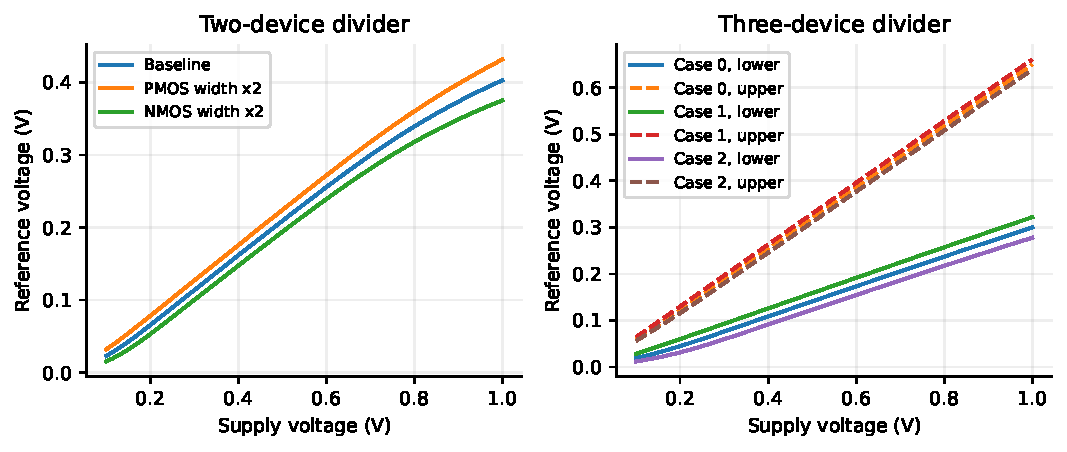
\includegraphics[width=\linewidth]{figures/reference_dividers.pdf}
\caption{兩種分壓參考的實際供應電壓掃描。三 MOS 的舊 2.1 V 目標在本次 1 V 電源下不可達。}
\end{figure}
\begin{center}\small\begin{tabular}{lrrrr}\toprule
Case & Temp. ($^\circ$C) & $V_{ref}$ (V) & $I_{DD}$ ($\mu$A) & $|A_{supply}|$ \\ \midrule
D05/C0 & 27 & 0.44410 & 311.95 & 0.01283 \\
D05/C1 & -20 & 0.37291 & 278.86 & 3.02680 \\
D05/C2 & 85 & 0.61066 & 420.07 & 0.47272 \\
D05/C3 & 27 & 0.21186 & 313.62 & 0.05349 \\
D05/C4 & 27 & 0.22662 & 203.08 & 1.97827 \\
\bottomrule\end{tabular}\end{center}
\begin{center}\small\begin{tabular}{lrrrr}\toprule
Case & Ramp ($\mu$s) & $V_{final}$ (V) & $t_{1\%}$ ($\mu$s) & $P_b$ ($\mu$W) \\ \midrule
D06/C0 & 1 & 0.44408 & 4.18 & 311.94 \\
D06/C1 & 30 & 0.44410 & 27.82 & 311.95 \\
D06/C2 & 1 & 0.37291 & 12.72 & 278.86 \\
D06/C3 & 1 & 0.61066 & 1.80 & 420.07 \\
D06/C4 & 1 & 0.44404 & 4.18 & 311.92 \\
\bottomrule\end{tabular}\end{center}
\begin{center}\small\begin{tabular}{lrrr}\toprule
Case & $I_{inj,pk}$ (nA) & $I_{inj,final}$ (nA) & $I_{core}$ ($\mu$A) \\ \midrule
D04/C0 & 222.739 & 3.8605 & 103.102 \\
D04/C1 & 3.978 & 3.8009 & 103.098 \\
D04/C2 & 0.087 & 0.0000 & 103.089 \\
D04/C3 & 0.023 & 0.0000 & 103.090 \\
\bottomrule\end{tabular}\end{center}
D01 的手算趨勢成立：提高 PMOS 相對驅動能力會提高輸出，提高 NMOS 能力會降低輸出。D03 在 5 k$\Omega$ 的 $V_{ref}=0.39866$ V，對應 $V_{ref}/R=79.732\,\mu$A；M5 量得約 $81.000\,\mu$A，差異需連同鏡像尺寸、$V_{DS}$ 與 body effect 解讀。

D05/C0 為基本條件；C1/C2 分別是 -20/85 $^\circ$C；C3 是 $R_3=3$ k$\Omega$；C4 是 $R_b=2$ k$\Omega$。D06/C0--C4 分別為基本、慢 ramp、低溫、高溫、啟動支路斷開。D04/C2--C3 斷開注入路徑後核心仍在這些名義模擬中啟動，不能把這個結果隱藏，也不能推論所有電源斜率與 corner 都不需要 startup。
\begin{figure}[htbp]\centering
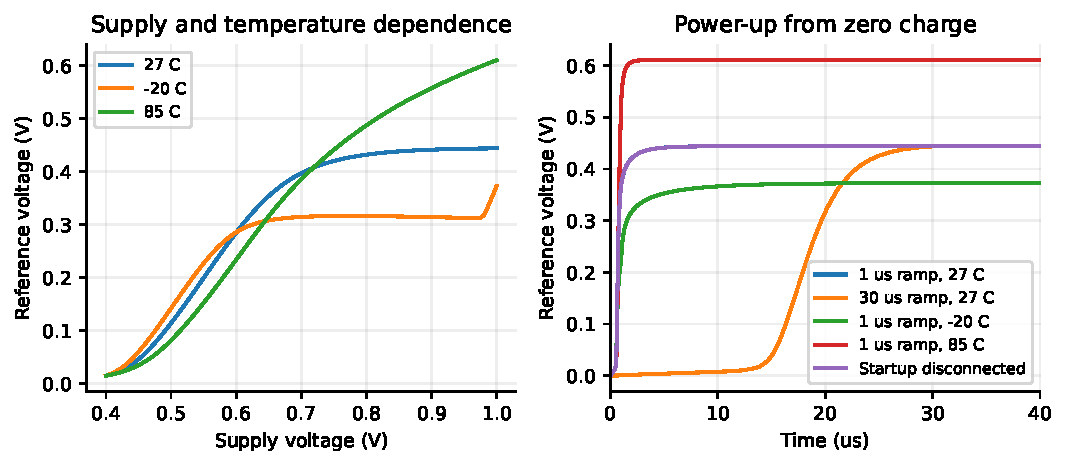
\includegraphics[width=\linewidth]{figures/reference_startup.pdf}
\caption{完整參考的 DC 溫度比較與啟動結果。溫度漂移和低溫 DC 分支轉換均如實保留。}
\end{figure}


\section{討論}
零電流解也是自偏壓迴路的平衡解；在 $I=0$ 附近，強反轉平方律的除法與非零解推導不成立。Startup 提供短暫電流以離開該狀態，之後應減弱以免污染參考。本次快速 ramp 的注入峰值約 222.7 nA、穩態約 3.86 nA；慢 ramp 沒有相同的尖峰，說明啟動具有路徑與斜率依賴。未加啟動仍能啟動的名義結果可能來自漏電與數值初始擾動，不能取代跨 corner 的啟動設計。

PDF 29 內文寫約 1.62 mV，圖的縱軸卻在 1.62 V 附近；本報告將它視為單位疑義，不以任一數值作本次 1 V 的必達目標。分壓電路依賴 $V_T$、遷移率和尺寸比；電阻退化可降低供應依賴，卻仍依賴 $\beta$、電阻及溫度。完整參考在 -20 至 85 $^\circ$C 仍有明顯漂移，不能宣稱具完整製程或溫度補償。若需溫度穩定度，應加入有明確溫度係數的互補項、電阻選型與調校，並取得可用 corner/溫度模型後驗證。

\section{結論}
講義各拓樸、啟動問題與補償討論均有對應程式和真實結果。1 V 下可得到約 0.444 V 的完整參考，但原製程幅度、全面製程補償與跨 corner 啟動可靠度不屬於已通過項目。

